\section{Производительность решения}

Целями следующих экспериментов является выявление эффекта произведенного использованием нескольких глобальных очередей и сопоставлением этих результатов с результатами использования нескольких рантаймов, для чего были поставлены следующие вопросы:

\begin{itemize}\label{quest}
    \item Будет ли пропускная способность рантайма с одной рабочей группой сопостовима с пропускной способностю исходного рантайма?
    \item Будет ли наблюдаться увеличение производительности при использовании большего количества рабочих групп?
    \item Будет ли пропускная способность рантайма с использованием нескольких рабочих групп сопостовима с пропускной способностью системы состоящей из такого же количества рантаймов?
    \item Будет ли наблюдаться изменение в производительности при изменении количества рабочих групп, если задачи акторы будут тривиальными конечными автоматами?
\end{itemize}

Эксперимент производился в окружении описанном в разделе~\ref{experiment_environment}.

\subsection{Ход исследования}

Количество потоков исполнителей и задач производителей было фиксировано и равномерно распределено между рантаймами или рабочими группами. Под количеством дубликатов имеется ввиду количество \verb|исходных рантаймов| или количество рабочих групп в составе одного \verb|модифицированного рантайма|.

На изображении~\ref{fig:tatlin:multi_rt_gp:eval} представлены результаты измерения основного сценария.

На изображении~\ref{fig:tatlin:rt_gp_spawn:eval} представлены результаты измерения сценария с тривиальными акторами.

\begin{figure}[H]
    \begin{center}
        \makebox[\textwidth]{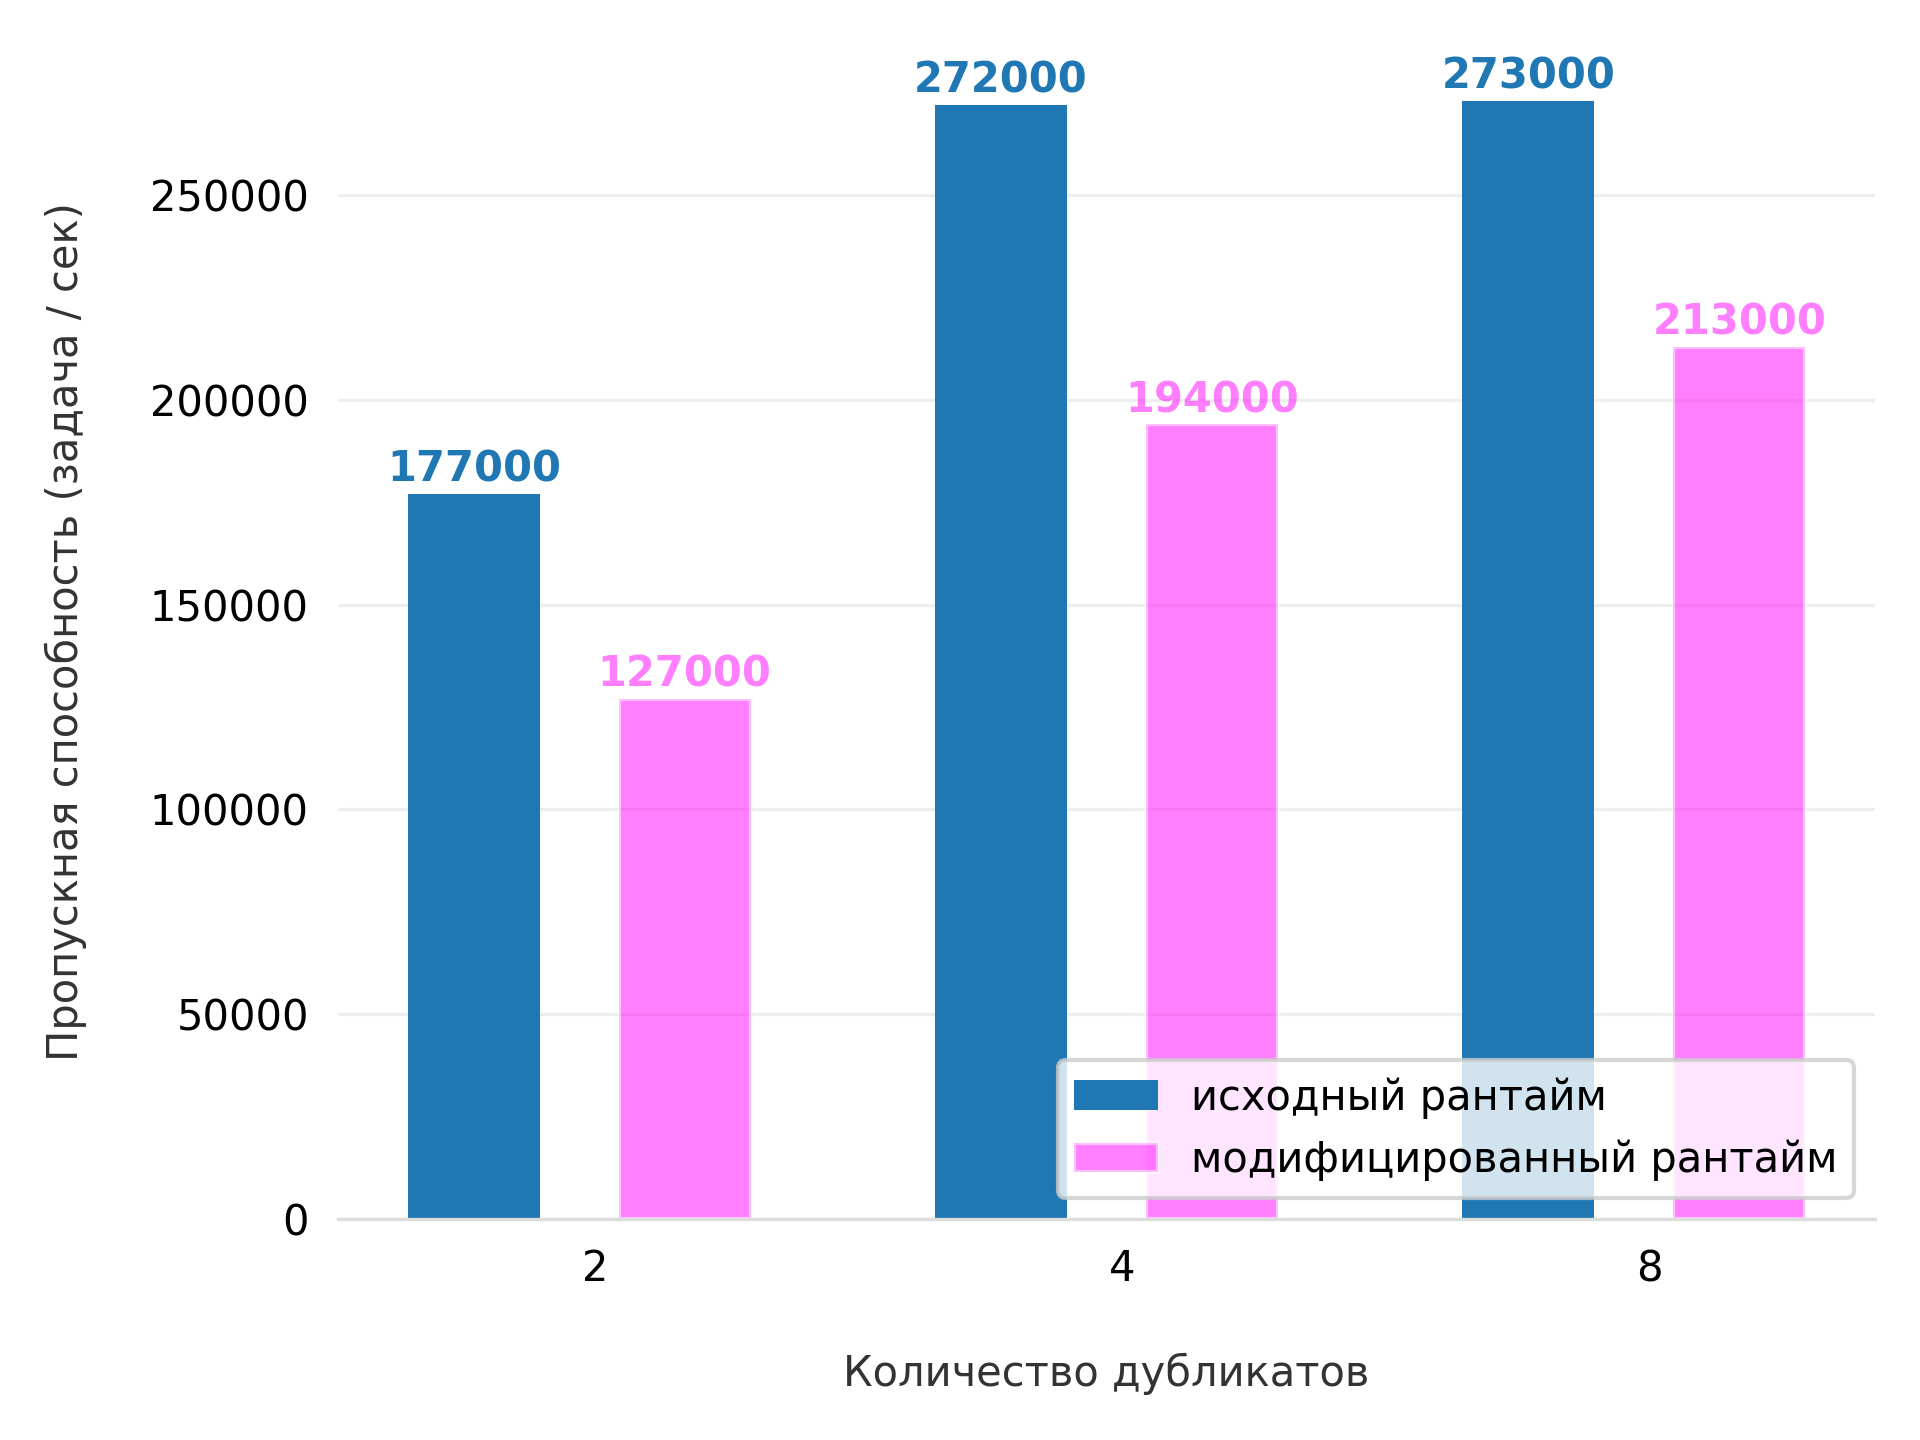
\includegraphics[scale=0.80]{pictures/rt_gp_nsapwner128_nspawn1000.png}}
    \end{center}

    \caption{Сравнение производительности исходного и модифицированного рантаймов в основном сценарии.}
    \label{fig:tatlin:multi_rt_gp:eval}
\end{figure}

\begin{figure}[H]
    \begin{center}
        \makebox[\textwidth]{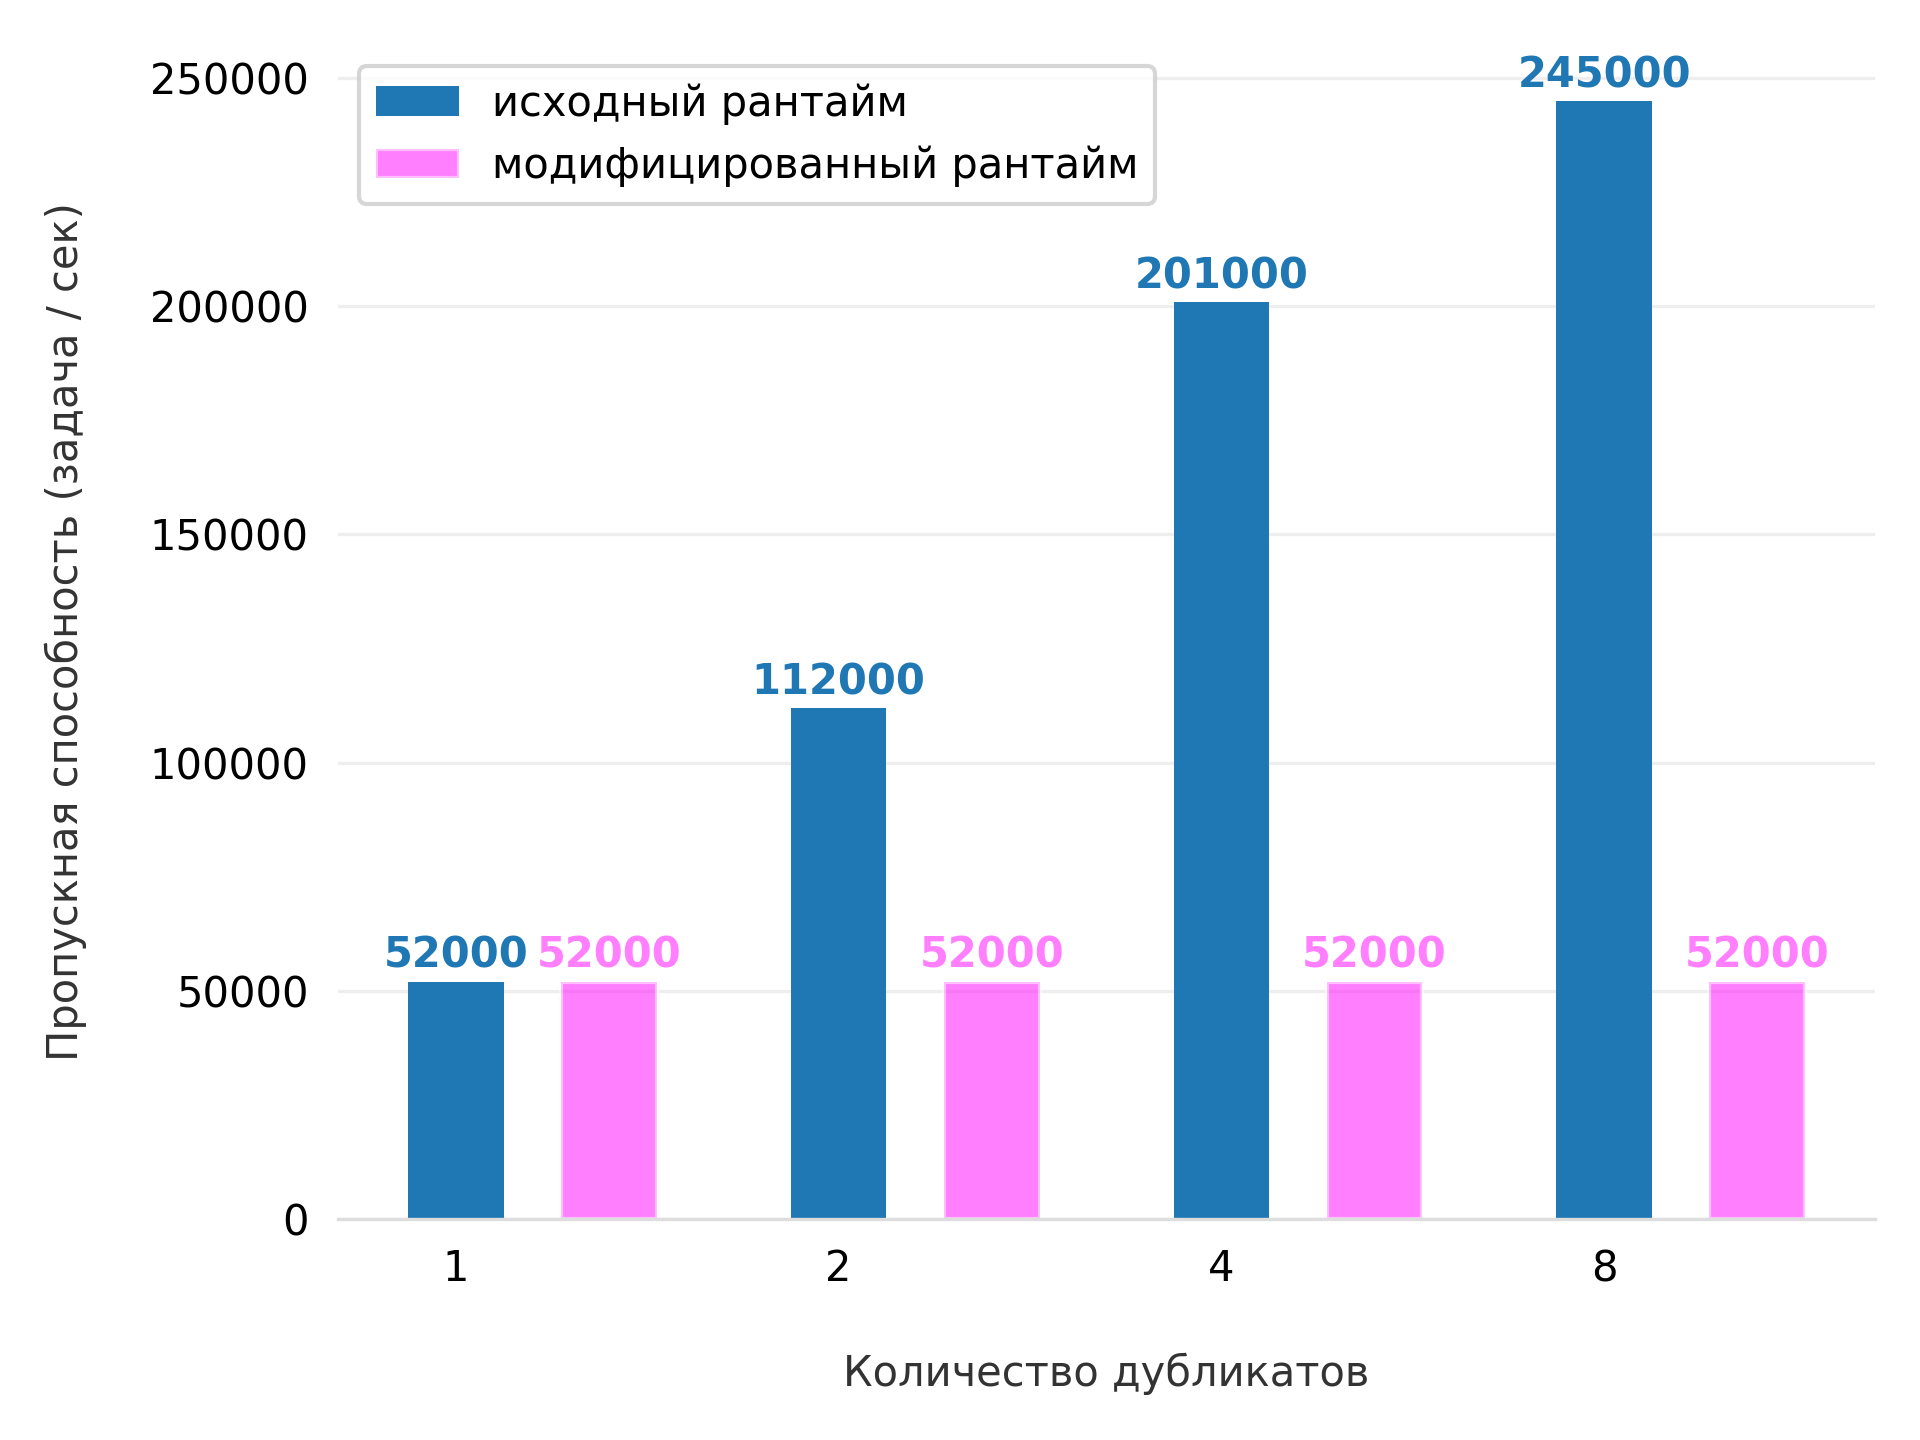
\includegraphics[scale=0.80]{pictures/rg_gp_spawn.png}}
    \end{center}

    \caption{Сравнение производительности исходного и модифицированного рантаймов в сценарии с тривиальными акторами.}
    \label{fig:tatlin:rt_gp_spawn:eval}
\end{figure}

Изображение~\ref{fig:tatlin:multi_rt_gp:eval} и~\ref{fig:tatlin:rt_gp_spawn:eval} демонстрирует ответы на поставленные выше вопросы~\ref{quest}:

\begin{itemize}
    \item Пропускная способность системы из одного рантайма и модифицированного рантайма, содержащего одну рабочую группу, демонстрируют одинаковую пропускную способность в обоих случаях.
    \item При увеличении количества глобальных очередей в системе, состоящей из одного рантайма, наблюдается увеличение пропускной способности в случае нетривиальных акторов. Это ожидаемый результат --- меньшее количество исполнителей конкурируют за глобальну и локальные очереди.
    \item Пропускная способность системы, состоящей из одного модифицированного рантайма, содержащего несколько очередей, меньше пропускной способности системы, состоящей из нескольких рантаймов. Это ожидаемый результат --- в системе, состоящей из отдельных рантаймов, требуется меньшее количество синхронизаций:
    \begin{itemize}
        \item Различные метрики, собираемые рантаймом реализованы с помощью атомарных счетчиков, разделяемых в случае одного рантайма.
        \item Многие структуры данных находятся близко в памяти, что может так же требовать дополнительной синхронизации между различными потоками.
    \end{itemize}
    \item В случае использования тривиальных акторов не наблюдается изменение пропускной способности при изменении количества групп в модифицированном рантайме, однако наблюдается при дубликации инстанцов рантайма. Это ожидаемый результат --- замыкания акторы создают большое количество единиц планирования, тем самым активно эксплуатируют планировщик, напротив, в процессе обработки тривиальных замыканий аллокация, регистрация в \verb|OwnedQueue| и деаллокация состовляет большую часть действий. Дублирование инстансов рантаймов позволяет избежать конукуренции за эти ресурсы, чего нельзя сказать об использовании одного рантайма с шардированным планировщиком, которые почти не участвует в процессе аллокации асинхронных замыканий.
\end{itemize}

\subsection{Выводы}

Шардирование планировщика многопоточного рантайма \verb|tokio| позволило увеличить пропускную способность системы создающей большое количество замыканий акторов, однако при аллокации тривиальных асинхронных задач пропускная способность не изменилась.
